\chapter{MATÉRIELS ET MÉTHODES}
Dans ce chapitre, nous présentons les matériels en détaillant la configuration matérielle ainsi que l’environnement de développement logiciel. Nous allons présenter aussi les méthodes et les techniques nécessaire pour la compréhension de ce mémoire.
\section{MATÉRIELS}
Dans cette section, nous allons examiner les diverses ressources matérielles et logicielles (tels que Jupiter, Google Colab, VSCode, Python, pandas, etc.) que nous avons utilisé durant notre projet.
\subsection{Outil Matériel}
Les analyses et traitements de données réalisés dans le cadre de cette étude ont été effectués principalement sur une machine avec les spécifications suivantes :

\begin{itemize}
	\item \textbf{Processeur :} Intel(R) Celeron(R) CPU N2840, 2.16GHz, 4 cœurs
	\item \textbf{Mémoire RAM :} 4 Go
	\item \textbf{Stockage :} HDD 250 Go
	\item \textbf{Système d'exploitation :} Windows 10
	\item \textbf{Carte graphique :} Intel HD Graphics
\end{itemize}

Ces caractéristiques matérielles, bien que modestes, ont suffi pour la gestion et l'analyse des données de cette étude. Cependant, le processus d'entraînement des modèles a nécessité une gestion efficace des ressources, notamment en optimisant le code pour éviter des surcharges de mémoire.

\subsection{Outil Logiciel}
Les logiciels et outils de programmation utilisés dans cette étude sont les suivants :

\begin{itemize}
	\item \textbf{Éditeurs de texte et environnements de développement :}
	\begin{itemize}
		\item Visual Studio Code (VSCode) : Utilisé pour l'édition du code et l'exécution de scripts Python.
		\item Jupyter Notebook : Principalement utilisé pour le prototypage rapide et l'exploration des données.
		\item Google Colab : Employé pour l'exécution de modèles sur des datasets volumineux grâce aux ressources cloud.
	\end{itemize}
	\item \textbf{Bibliothèques Python :}
	\begin{itemize}
		\item \textbf{Pandas :} Manipulation des données, notamment pour le nettoyage, la transformation, et l'agrégation des datasets.
		\item \textbf{BeautifulSoup :} Scraping des données climatiques depuis des sources en ligne, permettant de compléter les datasets de cas de Chikungunya avec des données météorologiques pertinentes.
		\item \textbf{NumPy :} Réalisation des calculs numériques, en particulier pour les opérations de vecteurisation et de manipulation de matrices, essentiels dans le prétraitement des données et les calculs statistiques.
		\item \textbf{Scikit-learn :} Développement et validation des modèles de machine learning, tels que la régression linéaire, les arbres de décision, et les modèles d'ensemble. Cette bibliothèque a été cruciale pour la mise en œuvre des modèles prédictifs.
		\item \textbf{Matplotlib et Seaborn :} Visualisation des données, permettant de créer des graphiques explicatifs pour mieux comprendre la distribution des données et les performances des modèles.
	\end{itemize}
	\item \textbf{Système de gestion de versions :}
	\begin{itemize}
		\item \textbf{Git :} Utilisé pour le contrôle des versions et la gestion collaborative du code. Chaque modification a été suivie et documentée, facilitant ainsi le travail en équipe et l'historisation des changements.
	\end{itemize}
\end{itemize}

%\textit{vanishing gradient}\footnote{Le \textit{vanishing gradient}

\section{Méthodes}
Cette section décrit les méthodes que nous avons utilisées.

\subsection{Collecte de données}
Les données utilisées dans cette étude proviennent de diverses sources fiables. 
\subsubsection{Données épidémiologiques}
\begin{itemize}
	\item Pour le \textbf{Tchad} : les données épidémiologiques ont été extraites d'un rapport~\cite{rapport2020oms} de l'Organisation Mondiale de la Santé (OMS) lors de l'émergence du Chikungunya en \textbf{2020}. Ce dataset couvre la période allant du \textit{12 août 2020} au \textit{10 novembre 2020}
	\item Concernant le \textbf{Brésil} : les données ont été recueillies à partir du site de mendeley\footnote{\url{https://data.mendeley.com/datasets/2d3kr8zynf/2}} . Cet ensemble de données présente des informations cliniques, \textbf{sociodémographiques} et de laboratoire relatives aux patients confirmés atteints de \textit{dengue} et de \textit{chikungunya}. Il couvre la période de \textbf{2013} à \textbf{2020}, mais pour cette thèse, nous avons restreint notre analyse à l'intervalle de \textbf{2013} à \textbf{2017}.
	\item Pour le \textbf{Paraguay} : les données ont été collectées via le site de la PAHO\footnote{\url{https://www3.paho.org/data/index.php/en/mnu-topics/chikv-en/550-chikv-weekly-en.html}} , qui rapporte les cas de Chikungunya en temps réel, avec des enregistrements hebdomadaires variant entre 2013 et 2017.
\end{itemize}
\subsubsection{Données climatiques}
Les données climatiques pour ces trois pays ont été obtenues à partir du site weatherandclimate\footnote{\url{http://weatherandclimate.com/}}, correspondant aux mêmes intervalles temporels que les cas de Chikungunya dans chaque pays. Ces données comprennent des paramètres tels que l'humidité, la température et les précipitations, essentiels pour étudier l'impact des conditions météorologiques sur la propagation de la maladie.

\subsection{Exploration et Préparation des Données}
L'exploration des données a débuté par une analyse des features climatiques, incluant l'\textbf{humidité}, la \textbf{température} et les \textbf{précipitations}. Cette étape visait à comprendre la distribution des données climatiques et leur variation au fil du temps.
\subsubsection{Préparation des Données}
La préparation des données pour le \textbf{Tchad} et le \textbf{Paraguay} a présenté des défis importants en raison du manque de données \textbf{suffisantes}.

\paragraph*{Nettoyage des données}
\begin{itemize}
	\item Pour le \textbf{Tchad} : les données disponibles couvrent une période limitée, du \textbf{14 août 2020} au \textbf{1er octobre 2020}.
	\item Pour le \textbf{Paraguay} : les données disponibles étaient à une fréquence irrégulière et ne couvraient pas l'intégralité des mois.
\end{itemize}

Pour pallier ces lacunes, nous avons envisagé plusieurs méthodes de traitement des données manquantes. Les méthodes sélectionnées sont les suivantes :

\begin{itemize}
	\item \textbf{Forward Fill} : Cette méthode consiste à propager les valeurs disponibles vers les valeurs manquantes situées ultérieurement dans le temps.
	\item \textbf{KNN Imputer} : Cette méthode utilise les k-plus proches voisins pour estimer les valeurs manquantes en se basant sur les données les plus proches.
\end{itemize}

\paragraph*{Feature Engineering}
\begin{itemize}
	\item[\space] Le \textit{feature engineering} est une technique qui consiste à créer de nouvelles variables (features) à partir des données brutes. Dans le cadre de notre étude, nous avons utilisé cette approche pour améliorer les données épidémiologiques du Brésil. En effet, lors de la collecte des données sur les cas de Chikungunya, nous avons rencontré un ensemble de données comprenant à la fois des patients testés positifs pour la dengue et pour le Chikungunya. Nous avons alors croisé les données des patients testés positifs pour le Chikungunya avec les dates de détection de leur maladie. Cela nous a permis de créer une nouvelle variable (feature) associant chaque cas à une date spécifique, ce qui a enrichi notre base de données épidémiologiques.
\end{itemize}

\subsubsection{Exploration des Données}
Dans cette section, nous allons explorer nos données de manière détaillée. Nous commencerons par présenter les entêtes des différents jeux de données, puis nous analyserons l'évolution du Chikungunya au fil du temps dans les pays étudiés. Enfin, nous mettrons en évidence les corrélations entre les features, en particulier les données climatiques et épidémiologiques.

\subsubsection*{Les Entêtes des Données}
\begin{itemize}
	\item \textbf{Entêtes des données climatiques} : La figure ci-dessous illustre les principales variables disponibles dans les jeux de données climatiques, qui incluent la date, la température, l'humidité et les précipitations.
	\begin{figure}[h!]
		\centering
		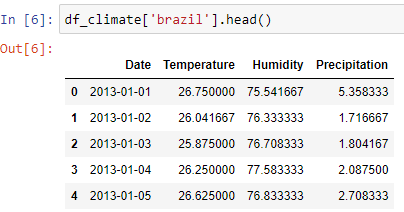
\includegraphics[width=0.5\linewidth]{images/climate_dataset_sample}
		\caption[Exemple d'entêtes des données climatiques]{Exemple d'entêtes des données climatiques}
		\label{fig:climatedatasetsample}
	\end{figure}
	
	\item \textbf{Entêtes des données épidémiologiques} : La figure suivante montre les principales variables présentes dans les jeux de données épidémiologiques, couvrant les cas de Chikungunya au fil du temps.
	\begin{figure}[h!]
		\centering
		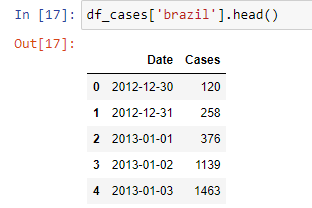
\includegraphics[width=0.5\linewidth]{images/cases_dataset_sample}
		\caption[Exemple d'entêtes des données épidémiologiques]{Exemple d'entêtes des données épidémiologiques}
		\label{fig:casesdatasetsample}
	\end{figure}
\end{itemize}

Ainsi, lorsque nous associons les données épidémiologiques aux données climatiques, l'entête du jeu de données résultant est illustrée dans la figure ci-dessous :
\begin{figure}[h!]
	\centering
	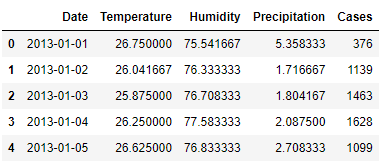
\includegraphics[width=0.7\linewidth]{images/dataset_sample}
	\caption{Exemple du dataset final combinant les données climatiques et épidémiologiques}
	\label{fig:datasetsample}
\end{figure}

\subsubsection*{Illustration de l'Évolution du Chikungunya}
\begin{itemize}
	\item \textbf{Cas du Tchad}\\
	L'émergence du virus au Tchad a été observée entre le \textbf{14 août 2020} et le \textbf{1er octobre 2020}.
	\begin{figure}[h!]
		\centering
		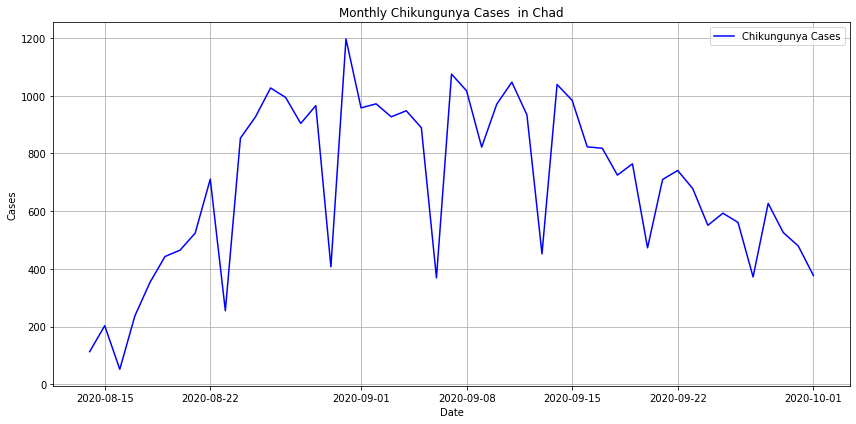
\includegraphics[width=0.6\linewidth]{images/case_chad}
		\caption[Évolution du Chikungunya au Tchad]{Évolution du Chikungunya au Tchad}
		\label{fig:casechad}
	\end{figure}
	
	\item \textbf{Cas du Brésil}\\
	L'épidémie au Brésil s'est étendue du \textbf{1er janvier 2013} au \textbf{31 décembre 2017}.
	\begin{figure}[h!]
		\centering
		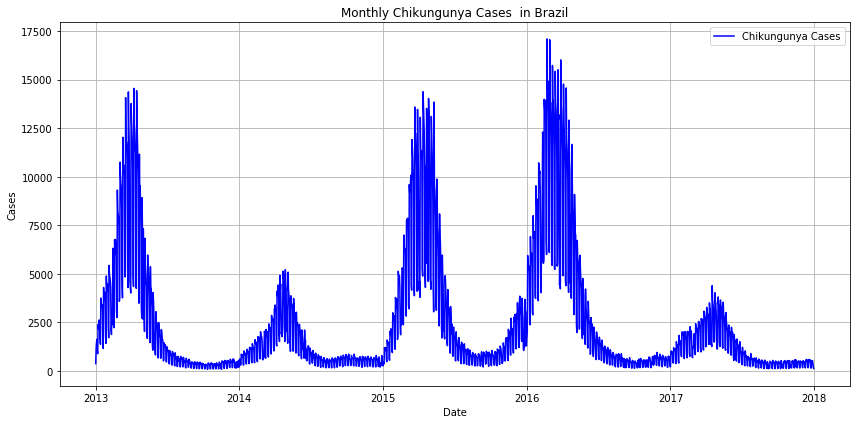
\includegraphics[width=0.6\linewidth]{images/case_brazil}
		\caption[Évolution du Chikungunya au Brésil]{Évolution du Chikungunya au Brésil}
		\label{fig:casebrazil}
	\end{figure}
	
	\item \textbf{Cas du Paraguay}\\
	L'épidémie au Paraguay a également été observée entre le \textbf{1er janvier 2013} et le \textbf{31 décembre 2017}.
	\begin{figure}[h!]
		\centering
		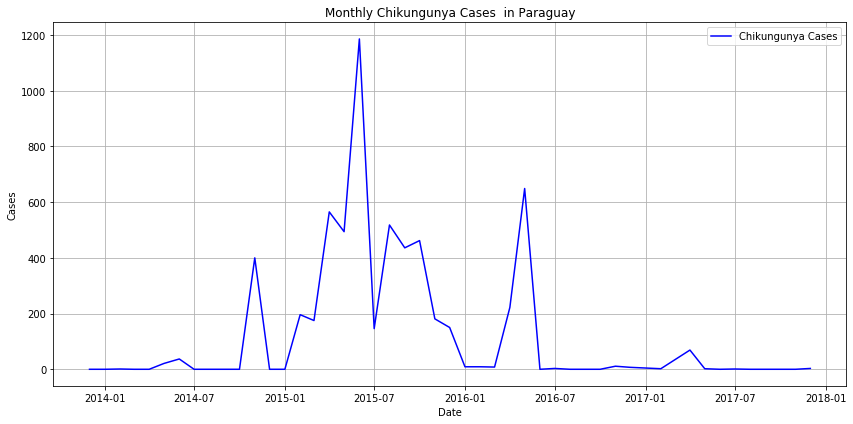
\includegraphics[width=0.6\linewidth]{images/case_paraguay}
		\caption[Évolution du Chikungunya au Paraguay]{Évolution du Chikungunya au Paraguay}
		\label{fig:caseparaguay}
	\end{figure}
\end{itemize}

\subsubsection*{Analyse de Corrélation}
L'analyse suivante explore la relation entre le nombre de cas de Chikungunya et les variables climatiques. 
\begin{figure}[h!]
	\centering
	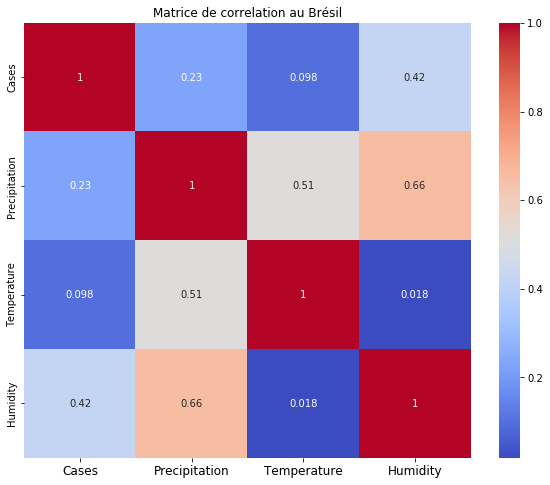
\includegraphics[width=0.5\linewidth]{images/case_correlation}
	\caption[Corrélation entre les variables climatiques et le nombre de cas]{Corrélation entre les variables climatiques et le nombre de cas}
	\label{fig:casecorrelation}
\end{figure}

L'exploration des données a également mis en évidence certaines anomalies, telles que des variations extrêmes ou des lacunes dans les enregistrements, nécessitant des ajustements méthodologiques spécifiques pour assurer la fiabilité des analyses subséquentes.


\subsection{Modèle prédictif}
Pour prédire les cas de chikungunya, nous avons choisi d'utiliser plusieurs modèles de régression supervisée. Cette approche nous permet de comparer les performances de différents algorithmes et d'obtenir des prévisions plus robustes grâce à un modèle d'ensemble. Les modèles choisis sont les suivants:

\subsubsection{Random Forest Regressor}
La \textbf{Random Forest Regression} en \textit{machine learning} est une technique d'\textbf{ensemble} capable d'exécuter des tâches de \textbf{régression} et de \textbf{classification} en utilisant plusieurs \textbf{arbres de décision} et une méthode appelée \textbf{Bootstrap and Aggregation}, communément connue sous le nom de \textit{bagging}. L'idée principale derrière cette approche est de combiner plusieurs arbres de décision pour déterminer le résultat final, plutôt que de se fier à un seul arbre de décision.

Dans une \textbf{Random Forest}, plusieurs arbres de décision servent de modèles d'apprentissage de base. On effectue un \textbf{échantillonnage aléatoire des lignes} (\textit{row sampling}) et des \textbf{caractéristiques} (\textit{feature sampling}) à partir du jeu de données, formant ainsi des sous-ensembles de données pour chaque modèle. Cette étape est appelée \textit{Bootstrap}.
\begin{figure}[h!]
	\centering
	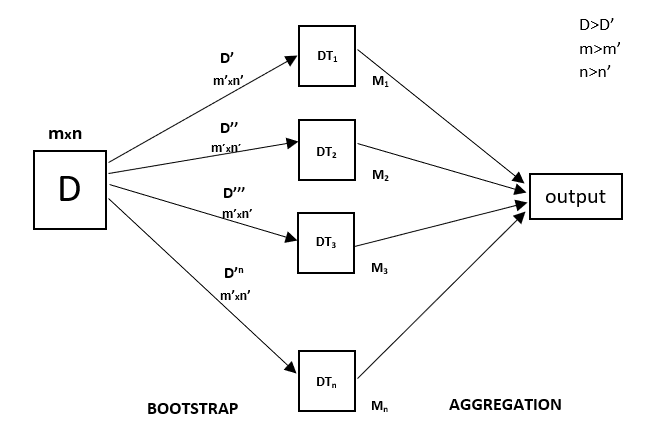
\includegraphics[width=0.4\linewidth]{images/schema_random_forest}
	\caption[Random Forest Regression]{Random Forest Regression working}
	\label{fig:schemarandomforest}
\end{figure}

\newpage
\subsubsection{XGBoost Regressor with Grid Search}

L'algorithme XGBoost  est un modèle de boosting qui utilise des arbres de décision comme base
\textbf{XGBoost} (Extreme Gradient Boosting) est une technique puissante pour construire des modèles de régression supervisée. Son efficacité repose sur sa \textbf{fonction objective} et ses \textbf{apprenants de base}. La fonction objective de \textbf{XGBoost} comprend une \textbf{fonction de perte} et un \textbf{terme de régularisation}. La fonction de perte mesure la différence entre les valeurs réelles et les valeurs prédites, ce qui indique à quel point les prédictions du modèle sont proches des valeurs réelles. Pour les problèmes de régression, la fonction de perte la plus courante dans \textbf{XGBoost} est \texttt{reg:linear}, tandis que pour la classification binaire, il s'agit de \texttt{reg:logistic}.Ce modèle est reconnu pour sa haute performance, particulièrement lorsqu'il est combiné avec une recherche en grille pour optimiser les hyperparamètres.


\paragraph*{Hyperparamètres:}
Les hyperparamètres du modèle ont été ajustés à l'aide de la recherche en grille (\textbf{Grid Search}) pour optimiser la performance qui seront illustré dans le chapitre 4.

\begin{figure}[h!]
	\centering
	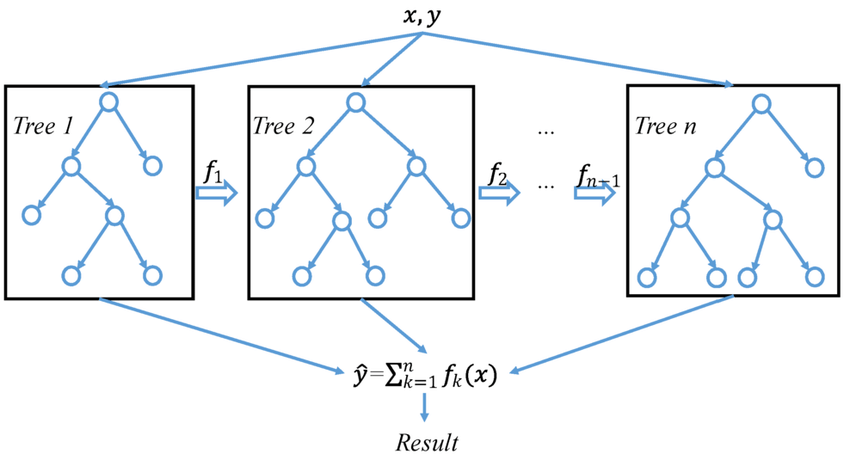
\includegraphics[width=0.5\linewidth]{images/schema_xgboost}
	\caption{Architecture Générale XGboost}
	\label{fig:schemaxgboost}
\end{figure}


\subsubsection{Ensemble Model (Voting Regressor)}

Pour tirer parti des forces de chaque modèle, nous avons implémenté un modèle d'ensemble, le \textbf{Voting Regressor}, qui combine les prédictions du \textit{Random Forest}, du \textit{XGBoost optimisé}, et d'une \textit{régression linéaire}. Ce modèle utilise une méthode de vote pondéré pour calculer la prédiction finale, offrant ainsi une plus grande stabilité et précision.

Un \textbf{Voting Regressor} peut être défini comme une méthode spéciale qui combine ou \textbf{ensemence} plusieurs modèles de régression et surpasse les modèles individuels qui le composent. Le concept mathématique du \textbf{Voting Regressor} est assez simple et très similaire à celui du \textbf{Voting Classifier}. Si l'on considère une foule de modèles de machine learning comme \(M_1, M_2,\dots , M_x\), alors chaque modèle \(M_n\) produira une prédiction \(P_n\) pour une donnée d'entrée \(I\). Maintenant, si nous passons ces prédictions à travers le \textbf{Voting Regressor}, la prédiction finale sera \(P_{\text{voting}}\). Nous pouvons alors choisir le mode de moyenne simple qui distribue uniformément le poids total à tous les modèles ou bien choisir des poids personnalisés pour chaque modèle, ce qu'on appelle la \textbf{moyenne pondérée}.

\textbf{Pour la moyenne simple :} 
\[
P_{\text{voting}}=\frac{1}{x}\sum_{n=1}^x{P_n}       
\]

\textbf{Pour la moyenne pondérée :} 
\[
P_{\text{voting}}=\sum_{n=1}^x (\text{wt}_{n} \cdot P_n)
\]
où \(\text{wt}_n\) sont les poids personnalisés assignés pendant le processus d'entraînement.

Mais l'expression ou le concept mathématique ne suffit pas à comprendre directement le \textbf{Voting Regressor}.


\begin{figure}[h!]
	\centering
	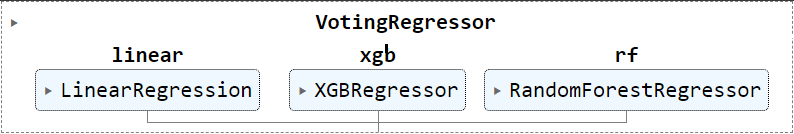
\includegraphics[width=0.7\linewidth]{images/schema_ensemble}
	\caption{Votting Regressor Architecture}
	\label{fig:schemaensemble}
\end{figure}
